% !TeX program = xelatex
\documentclass[UTF8]{beamer}

% -----------------------------------------------------------------------------
% Language support
% -----------------------------------------------------------------------------
\usepackage{xeCJK}

% -----------------------------------------------------------------------------
% Mathematics and tables
% -----------------------------------------------------------------------------
\usepackage{amsmath}
\usepackage{physics}
\usepackage{booktabs}
\usepackage{tabularx}

% -----------------------------------------------------------------------------
% Graphics and code listings
% -----------------------------------------------------------------------------
\usepackage{graphicx}
\usepackage{listings}
\lstset{
  basicstyle=\ttfamily,
  breaklines=true,
  columns=fullflexible,
  keepspaces=true,
  showstringspaces=false
}

% -----------------------------------------------------------------------------
% Colours and boxes
% -----------------------------------------------------------------------------
\usepackage{xcolor}
\usepackage{tcolorbox}

% -----------------------------------------------------------------------------
% Fonts
%   - palatino for Latin
%   - Noto Serif CJK SC for Chinese
%   - Inconsolata for mono
% -----------------------------------------------------------------------------
\usepackage[T1]{fontenc} 
\usepackage{palatino} 
\setCJKmainfont{Noto Serif CJK SC} % or other, see list below \setmonofont{Inconsolata}
\setmonofont{Inconsolata}

% Make math use the text font family by default
\def\mathfamilydefault{\rmdefault}

% -----------------------------------------------------------------------------
% 16:9 slide canvas
% -----------------------------------------------------------------------------
\usepackage[
  orientation=landscape,
  size=custom,
  width=16,
  height=9,
  scale=0.5
]{beamerposter}

% Compatibility fix for older Babel releases.
\makeatletter
\let\@@magyar@captionfix\relax
\makeatother

% -----------------------------------------------------------------------------
% Custom commands
% -----------------------------------------------------------------------------
\newcommand{\der}[2]{\frac{d #1}{d #2}}
\newcommand{\nder}[3]{\frac{d^{#1} #2}{d #3^{#1}}}
\newcommand{\pder}[2]{\frac{\partial #1}{\partial #2}}
\newcommand{\npder}[3]{\frac{\partial^{#1} #2}{\partial #3^{#1}}}

\newcommand{\overbar}[1]{%
  \mkern1.5mu\overline{\mkern-1.5mu#1\mkern-1.5mu}\mkern1.5mu%
}
\newcommand{\lined}{\overbar}
\newcommand{\perm}[2]{{}^{#1}\!P_{#2}}
\newcommand{\comb}[2]{{}^{#1}C_{#2}}
\newcommand{\intall}{\int_{-\infty}^{\infty}}
\newcommand{\Var}[1]{\text{Var}\left(#1\right)}
\newcommand{\E}[1]{\text{E}\left(#1\right)}
\newcommand{\define}{\equiv}
\newcommand{\diff}[1]{\mathrm{d}#1}

\newcommand{\empy}[1]{{\color{darkorange}\emph{#1}}}
\newcommand{\empr}[1]{{\color{cardinalred}\emph{#1}}}
\newcommand{\empbf}[1]{{\color{cardinalred}\bfseries #1}}

\newcommand{\examplebox}[2]{%
  \begin{tcolorbox}[colframe=darkcardinal,colback=boxgray,title=#1]
    #2
  \end{tcolorbox}
}

% -----------------------------------------------------------------------------
% Theme and deck-specific visual language
% -----------------------------------------------------------------------------
\usetheme{Stanford}
\beamertemplatenavigationsymbolsempty
\setbeamerfont{frametitle}{size=\large,series=\bfseries}
\setbeamerfont{title}{size=\LARGE,series=\bfseries}
\setbeamercolor{itemize item}{fg=darkcyan}
\setbeamercolor{itemize subitem}{fg=darkcyan}
\setbeamercolor{enumerate item}{fg=darkcyan}

\definecolor{okgreen}{RGB}{0,128,96}
\definecolor{warngold}{RGB}{188,122,25}
\definecolor{openrose}{RGB}{174,63,79}
\newcommand{\done}{\textcolor{okgreen}{\textbf{done}}}
\newcommand{\running}{\textcolor{warngold}{\textbf{running}}}
\newcommand{\open}{\textcolor{openrose}{\textbf{open}}}

\usepackage{multicol}
\setlength{\columnsep}{0.5cm}

% -----------------------------------------------------------------------------
% Presentation metadata
% -----------------------------------------------------------------------------
\title[DEGRACE companions: status]{\textbf{DEGRACE companions in MG-GLAM: status}}
\subtitle{What landed, what the products are, how they were verified, what the pilots say, what is left}

\author[C.-Z. Ruan]{\Large Cheng-Zong Ruan}

\institute[Durham University]{%
  
\includegraphics[height=0.72in]{durham_logo.png}\\[0.65ex]
  \small Institute for Computational Cosmology, Durham University
}
\date{17 October 2026 \quad\textcolor{coolgray}{\small merged into \texttt{cz}; plan in \texttt{docs/}}}

% -----------------------------------------------------------------------------
% Document
% -----------------------------------------------------------------------------
\begin{document}

\begin{frame}[plain]
  \titlepage
\end{frame}

% -----------------------------------------------------------------------------
\begin{frame}{\textbf{One week from plan to merged code}}
  \small
  \begin{itemize}
    \item \textbf{Scope} (plan of 16 Oct): 42 exact outputs per box (17 primary redshifts + 25 stations
      at $\Delta\chi = 256\,h^{-1}$Mpc), lens planes instead of snapshots, and the extra products of the
      brief: $\delta_L$, low-$k$ density and momentum modes, a hashed subsample, $f_R$ at halo centres.
    \item \textbf{Implemented} on \texttt{degrace-track-a} (17 commits, 53 files, +10.8k lines):
      items I1--I10; I11 (optional) not done.
    \item \textbf{Verified}: 180-check regression suite + four unit/integration scripts,
      six independent code reviews (0 blockers, 8 majors, all fixed), two pilots on ECOSMOG node 2.
    \item \textbf{Merged} into \texttt{cz} today (fast-forward, suite green on \texttt{cz}).
  \end{itemize}
  \examplebox{Take-away}{%
    Everything a companion run needs exists, is tested, is on the mainline and has run twice at $1024^3$.
    Three design decisions and one $0.5\,\%$ question remain.
  }
\end{frame}

% -----------------------------------------------------------------------------
\begin{frame}{\textbf{Status of the plan items}}
  \scriptsize
  \begin{tabularx}{\textwidth}{@{}l X l l@{}}
    \toprule
    item & what & status & evidence \\
    \midrule
    I1 & exact-$z$ scheduler accepts arbitrarily close output pairs & \done\ (\texttt{cz} ae4fa9d) & suite case 7 \\
    I2 & lens planes: 12 per output, $\Sigma/\bar\Sigma$ on $2048^2$ & \done & L1--L3 \\
    I3--I5 & input generator, \texttt{OutputSchedule.dat}, per-output classes & \done & cases 9, 4e; S2 (42 epochs = ECOSMOG to $10^{-7}$) \\
    I6 & provenance per box & partial & JSON lacks generator/LPT/seed (minor) \\
    I7 & $\delta_L(k)$ dump, route 1: in our FML IC generator & \done & V3, V7, V8; \texttt{run\_deltaL\_test.sh} \\
    I8 & low-$k$ $\delta_m$ and $(1+\delta)\mathbf{v}$ modes & \done & V1, V2, mode-by-mode \\
    I9 & ID-hashed quantised subsample, 1 in $M$ & \done & V5, V6; \texttt{run\_ic2pm\_test.sh} \\
    I10 & $f_R$ at BDM halo centres & \done & unit test + f(R) smoke case \\
    I11 & optional extras & \open & not started \\
    \midrule
    pilot & node 2 $\Lambda$CDM, $N_g = 2048$ & \done & verified, 0 FAIL \\
    pilot & node 2 f(R), extras + subsample + $f_R$ & \done & verified, 0 FAIL; 6 h 08 min \\
    \bottomrule
  \end{tabularx}
  \smallskip
  All flags default off: without the new \texttt{Init.dat} lines the code follows the \texttt{cz} path
  (review 2), apart from \texttt{OutputSchedule.dat} and an appended \texttt{Setup.dat} block.
\end{frame}

% -----------------------------------------------------------------------------
\begin{frame}{\textbf{Schedule and output classes (I1, I3--I5)}}
  \footnotesize
  \begin{columns}[T]
    \begin{column}{0.57\textwidth}
      \begin{itemize}
        \item \textbf{17 primary redshifts} $z = 0, 0.125, \ldots, 2$ ($\Delta z = 0.125$), common to all cosmologies.
        \item \textbf{25 stations} at comoving distance $\chi = 256\,k\;h^{-1}$Mpc, $k = 1\ldots25$, from the run's own
          flat matter\,+\,$\Lambda$ $\chi(a)$ (no radiation, $c/H_0 = 2997.92458\,h^{-1}$Mpc);
          \texttt{gen\_inputs.py} reproduces every ECOSMOG list to $10^{-7}$.
        \item \texttt{\#outputs = -42}: every epoch is hit exactly (a step moved onto it or inserted); pairs closer
          than 0.5\,\% are allowed. Pilot: 181 steps = 163 ladder + 18 inserted, $\mathrm{d}a_0 = 6\times10^{-4}$ from $z = 49$.
        \item \texttt{OutputSchedule.dat}: one line per output: step (= snapshot number), $a$, $z$, $\chi$, exact, class.
        \item \textbf{Class 1} (full): $P(k)$, planes, BDM catalogue, $f_R$ at haloes, $\delta_m$ and momentum cubes,
          subsample; \textbf{class 2} (station): $P(k)$ and planes. Pilots 17 + 25; production: all 42 class 1.
      \end{itemize}
    \end{column}
    \begin{column}{0.41\textwidth}
      \scriptsize
      \begin{tabular}{@{}rrrrcc@{}}
        \toprule
        step & $a$ & $z$ & $\chi$ & exact & class \\
        \midrule
        57  & 0.10275 & 8.732 & 6400.0 & 1 & 2 \\
        63  & 0.11832 & 7.452 & 6144.0 & 1 & 2 \\
        105 & 0.33333 & 2.000 & 3625.9 & 1 & 1 \\
        106 & 0.33796 & 1.959 & 3584.0 & 1 & 2 \\
        127 & 0.50000 & 1.000 & 2312.7 & 1 & 1 \\
        128 & 0.50128 & 0.995 & 2304.0 & 1 & 2 \\
        152 & 0.72727 & 0.375 & 1024.9 & 1 & 1 \\
        153 & 0.72747 & 0.375 & 1024.0 & 1 & 2 \\
        181 & 1.00000 & 0.000 & 0.0    & 1 & 1 \\
        \bottomrule
      \end{tabular}
      \\[1ex]
      \scriptsize Node 2 ($\Omega_m = 0.3$), $\chi$ in $h^{-1}$Mpc. Epochs equal the pinned ECOSMOG list to $10^{-7}$;
      steps 105/106, 127/128, 152/153 are the close pairs.
    \end{column}
  \end{columns}
\end{frame}

% -----------------------------------------------------------------------------
\begin{frame}{\textbf{What a box writes: files per output}}
  \scriptsize
  \begin{tabularx}{\textwidth}{@{}>{\raggedright\arraybackslash}p{0.28\textwidth} >{\raggedright\arraybackslash}X >{\raggedright\arraybackslash}p{0.19\textwidth} >{\raggedright\arraybackslash}p{0.12\textwidth}@{}}
    \toprule
    file (\texttt{<step>} = snapshot, box 0001) & content & $1024^3$, $N_g = 2048$ (pilots) & $2048^3$, $N_g = 4096$ \\
    \midrule
    \texttt{PowerDM.R/log.<step>.0001.dat} & $P(k)$ on the $N_g$ mesh, linear / log bins, raw CIC & 41 KB & 80 KB \\
    \texttt{LensPlanes.<step>.0001.bin/.meta} & 12 planes of $\Sigma/\bar\Sigma$, $N_{\rm lens}^2$ float32 & 201 MB ($2048^2$) & 805 MB ($4096^2$) \\
    \texttt{CatshortV.<step>.0001.DAT} / \texttt{.bin} + \texttt{.meta} & BDM haloes (in \texttt{CATALOGS/}): text, 24 columns; binary twin, 96 B per halo (\texttt{CatalogueFormat}) & 0.1--0.3 GB (binary $\tfrac13$) & 0.3--0.4 GB (binary $\tfrac13$) \\
    \texttt{deltam.<step>.0001.bin/.meta} & $\tilde\delta_m(\mathbf{k})$ cube, $k_c = 1.5$ & 469 MB & 469 MB \\
    \texttt{mom\_x,y,z.<step>.0001.bin/.meta} & $[(1+\delta)v_i]^{\sim}(\mathbf{k})$ cubes, $k_c = 0.75$ & $3\times59$ MB ($3\times138$ at $k_c = 1$) & same \\
    \texttt{Subsample.<step>.0001.bin/.meta} & 1 in $M = 100$ particles, int16 & 129 MB & 1.03 GB \\
    \texttt{fR\_halo.<step>.0001.bin/.meta} & $(f_R^{\rm centre}, f_R^{\rm mean})$ per halo & 9 MB (1.1 M haloes) & $\sim$30 MB \\
    \texttt{<IC prefix>\_deltaL.bin/.meta} & $\tilde\delta_L(\mathbf{k})$ cube, once per box, from the IC job & 469 MB & 469 MB \\
    \texttt{OutputSchedule.dat}, \texttt{timing.log} & schedule; per-step timing (with \texttt{Run.log}) & KB & KB \\
    \bottomrule
  \end{tabularx}
  \smallskip
  \footnotesize
  \begin{itemize}
    \item No particle snapshots (\texttt{iSave = 0}). Per box: 9.1 GB ($\Lambda$CDM pilot, no extras), 25 GB (f(R) pilot, extras at the 17 primaries); with the extras at
      all 42 outputs $\approx 40$ GB at $1024^3$ and $\approx 130$ GB at $2048^3$ (13 TB for 100 boxes).
  \end{itemize}
\end{frame}

% -----------------------------------------------------------------------------
\begin{frame}{\textbf{Conventions shared by every product}}
  \footnotesize
  \begin{itemize}
    \item \textbf{Epochs.} Positions at the output $a$ ($a_x = a$); velocities half a step behind, $a_v = a - \Delta a/2$
      with $\Delta a$ the step just taken (leapfrog). Every sidecar records \texttt{step, a, z, a\_x, a\_v}. The legacy
      BDM catalogue converts its velocities with $1/a$ instead of $1/a_v$ (0.3--0.8\,\% low; decision pending).
    \item \textbf{Units.} Comoving $h^{-1}$Mpc, peculiar velocities in km/s, masses in $h^{-1}M_\odot$; axes follow the
      particle $x, y, z$ of the catalogue (\texttt{axis\_map}).
    \item \textbf{Fourier.} $\tilde\delta(\mathbf{k}) = N^{-3}\sum_{\mathbf{x}}\delta(\mathbf{x})\,e^{-i\mathbf{k}\cdot\mathbf{x}}$,
      $\mathbf{k} = (2\pi/L)(i_x, i_y, i_z)$, $P(k) = L^3\langle|\tilde\delta|^2\rangle$; grid node $i$ at $(i-1)L/N$.
    \item \textbf{Mode cube.} $|i_x|, |i_y| \le n$, $0 \le i_z \le n$ with $n = \lfloor k_c L/2\pi\rfloor$; the Hermitian-redundant
      $i_z = 0$ modes are kept, $\mathbf{k} = 0$ is zero; $(2n+1)^2(n+1)$ complex64 values.
    \item \textbf{Layout.} Fortran \texttt{C(0:n,-n:n,-n:n)}, $i_z$ fastest; numpy
      \texttt{fromfile(f, '<c8').reshape(2n+1, 2n+1, n+1)[ix+n, iy+n, iz]}.
    \item \textbf{Mass assignment.} CIC on $N_{\rm dep}$ nodes, never deconvolved inside GLAM; \texttt{assignment},
      \texttt{N\_dep} and \texttt{interlaced = false} are recorded and offline code divides by $W_{\rm CIC}$.
    \item \textbf{Sidecar keys.} \texttt{product, format, layout, fourier\_norm, modes, n, k\_c, N\_dep, N\_grid, N\_row, N\_p,
      Box, units, D\_code(a)} (the code's flat matter\,+\,$\Lambda$ growth, $D(1) = 1$), \texttt{Omega\_m, Omega\_L, hubble,
      MG\_flag, MG\_model, fR0}, and \texttt{header} (the PM header: \texttt{ic2pm} velocity epoch, lattice tag \texttt{IDx}/\texttt{IDz}).
  \end{itemize}
\end{frame}

% -----------------------------------------------------------------------------
\begin{frame}{\textbf{Lens planes (I2): definition, cost, checks}}
  \footnotesize
  \begin{columns}[T]
    \begin{column}{0.58\textwidth}
      \begin{itemize}
        \item \textbf{Definition.} For projection axis $X$ and slab $s$ of depth $L/N_{\rm slab} = 256\,h^{-1}$Mpc, pixel
          $(i,j)$ is the mean of $1+\delta$ over the slab column and the pixel block, i.e. $\Sigma_s(i,j)/\bar\Sigma$ with
          $\bar\Sigma = \bar\rho_m\times$ depth; $\delta$ from the CIC deposit on $N_g$, not deconvolved. Each plane
          averages to 1 by construction.
        \item \textbf{Layout.} 12 planes in the order $X_1\ldots X_4, Y_1\ldots Y_4, Z_1\ldots Z_4$; $X$-planes indexed
          $(y, z)$, $Y$ $(x, z)$, $Z$ $(x, y)$; pixel $(i,j)$ covers $[(i-1), i)\,L/N_{\rm lens}$; float32,
          column-major; block average when $N_{\rm lens} < N_g$.
        \item \textbf{Offline use.} $\kappa = \tfrac{3}{2}\Omega_m (H_0/c)^2 \sum_{\rm planes}
          \frac{\chi(\chi_s-\chi)}{\chi_s\,a}\,(\Sigma/\bar\Sigma - 1)\,\Delta\chi$, $\Delta\chi = 256\,h^{-1}$Mpc.
        \item \textbf{Cost.} 1.8 s per output, the 201 MB write 12 s: $< 1\,\%$ of a run.
      \end{itemize}
    \end{column}
    \begin{column}{0.40\textwidth}
      \scriptsize
      \begin{tabular}{@{}ll@{}}
        \toprule
        check & result \\
        \midrule
        L1 mass conservation per axis & $10^{-7}$ \\
        L2 vs \texttt{ProjectDENSIT} & $10^{-5}$ \\
        L2 $36^2$ = block mean of $72^2$ & $10^{-5}$ \\
        L3 $P_{2D}$ vs projected $P_{3D}$ & $3\sigma$ per ring; 3--7\,\% \\
        pilots: plane means & $1 \pm 10^{-7}$ \\
        pilots: $\Sigma/\bar\Sigma$ range at $z = 0$ & 0.10--51 \\
        \bottomrule
      \end{tabular}
      \\[1ex]
      \examplebox{Open question for Baojiu}{%
        \scriptsize Plane normalisation ($\Sigma/\bar\Sigma$ vs $\Sigma$); do the stations also need halo catalogues?
      }
    \end{column}
  \end{columns}
\end{frame}

% -----------------------------------------------------------------------------
\begin{frame}{\textbf{Fourier dumps, subsample, $f_R$ at haloes (I8--I10)}}
  \scriptsize
  \begin{tabularx}{\textwidth}{@{}l X l@{}}
    \toprule
    product & what & verified \\
    \midrule
    \texttt{deltam} & $\delta_k = N^{-3}\sum_x \delta(x)e^{-ik\cdot x}$, cube $|k_i| \le k_c = 1.5$, CIC on $N_g$,
      complex64 $C(0{:}n,-n{:}n,-n{:}n)$ & V1 layout; V2 $=$ \texttt{PowerDM.R} to $10^{-4}$ \\
    \texttt{mom\_x,y,z} & $(1+\delta)\,v$ on $N_{\rm dep} = N_g/2$, $v$ at $a_v = a - \mathrm{d}a/2$,
      $k_c = 0.75$ (below $k_{N,\rm dep}/4$: no interlacing) & V6; mode by mode vs decoded particles $7\times10^{-5}$ \\
    \texttt{Subsample} & keep 1 in $M$ by splitmix64(ID $\oplus$ salt), int16 positions and velocities,
      deterministic across twins, threads, restarts & V5 ($10^7$ IDs), V6 \\
    \texttt{fR\_halo} & $f_R = f_{R,\rm bg}(a_{\rm old})\,u^{n+1}$ at every BDM centre & unit test; f(R) smoke case \\
    \bottomrule
  \end{tabularx}
  \smallskip
  \small
  \begin{itemize}
    \item Storage at $1024^3$ per output: $\delta_m$ 0.47 GB, momentum 0.18 GB ($k_c = 0.75$; 0.41 at 1.0), subsample ($M=100$) 0.13 GB.
    \item From the review: \texttt{ic2pm} places every particle at array index = Gadget ID and tags the
      lattice order (\texttt{IDz} 2LPTic, \texttt{IDx} FML) in the PM header, so the subsample index gives
      the Lagrangian position.
  \end{itemize}
\end{frame}

% -----------------------------------------------------------------------------
\begin{frame}{\textbf{Definitions: density, momentum and $\delta_L$ cubes (I7, I8)}}
  \footnotesize
  \begin{itemize}
    \item \texttt{deltam}: $\delta(\mathbf{x}) = n(\mathbf{x})/\bar n - 1$ from the CIC deposit of the output positions on
      $N_{\rm dep} = N_g$, forward FFT, cube $|k_i| \le k_c = 1.5\,h\,\mathrm{Mpc}^{-1}$ ($n = 244$ at $L = 1024$: 0.47 GB).
      Offline $P_{mm}(k) = L^3\langle|\tilde\delta_m/W_{\rm CIC}|^2\rangle$ equals \texttt{PowerDM.R} bin by bin to $10^{-4}$ (V2).
    \item \texttt{mom\_x,y,z}: $p_i(\mathbf{x}) = \bar n_{\rm cell}^{-1}\sum_p v_{i,p}\,W_{\rm CIC}(\mathbf{x}-\mathbf{x}_p)
      = (1+\delta)\,v_i$, $v$ the peculiar velocity in km/s at $a_v$; deposit on $N_{\rm dep} = N_g/2$, $k_c = 0.75$ by
      the rule $k_c \le k_{N,\rm dep}/4 = \pi N_{\rm dep}/4L$ (no interlacing; the f(R) pilot used 1.0).
      At linear $k$, $\tilde v_i \simeq \tilde p_i$.
    \item \texttt{deltaL}: the IC generator's Gaussian field at $z_{\rm ini}$ divided by $D(a_{\rm ini})$ (flat
      matter\,+\,$\Lambda$, $D(1) = 1$), i.e. the linear field at $a = 1$; written before any LPT displacement, same cube
      and layout as \texttt{deltam}, identical for a $\Lambda$CDM/f(R) twin pair (one IC file). Sidecar adds
      \texttt{seed, z\_ini, D\_gen(a\_ini), pofk\_file, lpt\_order, fix\_amplitude, lattice} (particles at $iL/N_p$,
      ID $= 1 + i_x + N_p(i_y + N_p i_z)$) and the cube rms.
    \item \textbf{Uses.} Halo propagator $\Gamma_h(k|M) = \sum\mathrm{Re}[\tilde\delta_h\tilde\delta_L^*]/\sum|\tilde\delta_L|^2$
      without cosmic variance; matter propagator $G_m = P_{mL}/P_L$; growth check
      $\langle\tilde\delta_m/W_{\rm CIC}/\tilde\delta_L\rangle = D_{\rm code}(a)$ (0.9997--1.0012 at $k \le 0.15$, V3);
      halo--momentum cross spectra; environment and tidal fields at $R \ge 3/k_c$.
    \item \textbf{Caveat.} Compare dumps with binned means and cross-correlations, not single-mode ratios (CIC of lattice
      particles is not linear in the displacement; phase scatter $\sim k\Delta/2$ at early times).
  \end{itemize}
\end{frame}

% -----------------------------------------------------------------------------
\begin{frame}{\textbf{Definitions: particle subsample (I9) and $f_R$ at haloes (I10)}}
  \scriptsize
  \begin{columns}[T]
    \begin{column}{0.56\textwidth}
      \textbf{\texttt{Subsample}}
      \begin{itemize}
        \item ID $=$ 0-based lattice index $i + N(j + Nk)$ ($i$ along $x$ for FML ICs, tag \texttt{IDx}; Baojiu's 2LPTic
          files are $k$-fastest, \texttt{IDz}); \texttt{ic2pm} places particle = Gadget ID. Lagrangian position
          $\mathbf{q} = (i, j, k)\,L/N$.
        \item Keep iff \texttt{splitmix64(ID xor SALT) mod M = 0}, \texttt{SALT = 0x5EED00DE6C0A2026}, $M = 100$:
          the same particles at every output and in both twins; $n_{\rm sel} = 10\,741\,150 = N/100$ to 0.03\,\%.
        \item Stored in increasing ID: the $k$-th particle is the $k$-th ID passing the rule (IDs implicit).
        \item int16 quantisation: $q = \lfloor 65536\,x/L\rfloor - 32768$, decode $x = (q + 32768 + 0.5)\,L/65536$
          ($\Delta x = 15.6\,h^{-1}$kpc); $s = \mathrm{nint}(v/\Delta v)$, $\Delta v = 0.25$ km/s, clipped at
          $\pm32767$ (count in the sidecar, 0 in the pilot); $v$ peculiar at $a_v$.
        \item Layout: \texttt{qx, qy, qz, vx, vy, vz}, $n_{\rm sel}$ each, contiguous; 12 B per particle.
      \end{itemize}
    \end{column}
    \begin{column}{0.42\textwidth}
      \textbf{\texttt{fR\_halo}} (f(R) runs, \texttt{MG\_model = 1})
      \begin{itemize}
        \item One float32 pair $(f_R^{\rm centre}, f_R^{\rm mean})$ per catalogue row, in \texttt{CatshortV} order.
        \item $f_R^{\rm centre}$: CIC interpolation of $f_R$ at the BDM centre; $f_R^{\rm mean}$: mean over the mesh cells
          whose centres lie within $R_{\rm vir}$ (equal to the centre value below half a cell).
        \item $f_R(\mathbf{x}) = f_{R,\rm bg}(a_{\rm old})\,u(\mathbf{x})^{n+1}$, $u$ the solver field (scalar field over its
          background value) at the pre-step epoch $a_{\rm old}$;
          $f_{R,\rm bg}(a) = f_{R0}\,[R_0/R(a)]^{n+1}$, $R(a) = 3(\Omega_m a^{-3} + 4\Omega_\Lambda)$.
        \item Sidecar: $f_{R0}$, $n$, $a_{\rm old}$, $f_{R,\rm bg}(a_{\rm old})$, catalogue name and row count.
      \end{itemize}
    \end{column}
  \end{columns}
\end{frame}

% -----------------------------------------------------------------------------
\begin{frame}{\textbf{$\delta_L$ from the IC generator (I7, route 1)}}
  \small
  \begin{columns}[T]
    \begin{column}{0.47\textwidth}
      \begin{itemize}
        \item The FML generator writes \texttt{<prefix>\_deltaL.bin/.meta}: its Gaussian field at $z_{\rm ini}$
          divided by $D(a_{\rm ini})$, same layout and convention as \texttt{deltam}; $k_c = 1.5$, 0.47 GB.
        \item Lua: \texttt{write\_deltaL}, \texttt{deltaL\_kc}; on in the production input. Costs 1 s.
        \item Baojiu's ICs and the legacy pilots are out of scope (decision of 17 Oct).
      \end{itemize}
    \end{column}
    \begin{column}{0.51\textwidth}
      \scriptsize
      \begin{tabular}{@{}ll@{}}
        \toprule
        check & result \\
        \midrule
        Zel'dovich: $\delta_L = -i\,k\cdot\Psi(k)/D$ & every mode to $10^{-3}$ \\
        2LPT ICs & residual $8\times10^{-3}$ (2nd order) \\
        wrong axis / sign / half cell & off by $10^4\times$ \\
        V3: ratio to $D(a)$, $k \le 0.15$ & 0.9997--1.0012 \\
        V3: cross-correlation, $k \le 0.05$ & 0.99998 \\
        V3: coordinate offset per axis & $\le 0.03\,h^{-1}$Mpc \\
        V7: 1/2/4 MPI ranks & identical md5 \\
        \bottomrule
      \end{tabular}
    \end{column}
  \end{columns}
  \examplebox{Lesson}{%
    CIC density of particles sitting on grid nodes is not linear in the displacement (phase scatter
    $\sim k\Delta/2$ per mode at early times): compare dumps with binned means and cross-correlations.
  }
\end{frame}

% -----------------------------------------------------------------------------
\begin{frame}{\textbf{Definitions: BDM halo catalogue and $P(k)$ (legacy products)}}
  \scriptsize
  \begin{itemize}
    \item \texttt{CATALOGS/CatshortV.<step>.0001.DAT}: text, 8 header lines (PM header with the \texttt{ic2pm} epoch and
      lattice tag, $a$ and $\Delta a$, step, $N_{\rm row}$, $N_g$, cosmology, buffer width, mass of the smallest particle,
      overdensity limit), then one row per halo with 24 columns:
      $x, y, z$ [$h^{-1}$Mpc]; $V_x, V_y, V_z$ [km/s]; $M_{\rm bound}$, $M_{\rm tot}$ [$h^{-1}M_\odot$]; $R_{\rm vir}$
      [$h^{-1}$kpc]; $V_{\rm rms}$, $V_{\rm circ}$ [km/s]; row index; $c_{\rm vir}$; $N_{\rm part}$; distinct/sub flag;
      $X_{\rm off}$; $2K/E_p - 1$; spin $\lambda$; RadRMS; $b/a$, $c/a$; major-axis direction $(x, y, z)$.
    \item \textbf{Binary twin} (\texttt{CatalogueFormat = text|binary|both} in \texttt{BDM.config}, compiled default binary
      since 2026-10-18, \texttt{text} or \texttt{both} on request; 2026-10-17/18): \texttt{CatshortV.<step>.0001.bin}, 96-byte little-endian records
      holding the same 24 columns (22 float32 + 2 int32), same rows and order, lossless; $3\times$ smaller apparent,
      $\approx 40\,\%$ on disk (this Lustre compresses text $1.9\times$); sidecar \texttt{.meta} with columns, units,
      rows, $a$, $a_v$, $\Delta a$, cosmology, $m_p$, \texttt{MassMin}, $\Delta_{\rm vir}$, definitions. Reader:
      \texttt{python/glamio} (\texttt{read\_catalogue}). \texttt{BDM.config} is validated at start-up.
    \item \textbf{Halo definition (BDM).} Centre = density peak refined by centre-of-mass iterations; $R_{\rm vir}$ = the
      spherical-overdensity radius at the Bryan--Norman $\Delta_{\rm vir}$ relative to the mean ($338$ at $z = 0$, 203 at
      $z = 1$ for $\Omega_m = 0.3$) plus a resolution correction of up to 0.75 cells; $M_{\rm bound}$ = bound mass inside the
      uncorrected radius, $M_{\rm tot}$ = all mass inside $R_{\rm vir}$; \texttt{MassMin} $= 10^{11}$ raised to 20 particles
      ($1.7\times10^{12}\,h^{-1}M_\odot$ at $1024^3$); rows in peak order, not by mass; velocities converted with $1/a$
      (low by $a_v/a$, decisions frame).
    \item \texttt{PowerDM.R.<step>.0001.dat}: 2 header lines ($a$, step, $z$, $N_g$, $k_{\rm Ny} = \pi N_g/L$), then
      bin, $k$ [$h\,\mathrm{Mpc}^{-1}$], number of modes, $P$ [$(h^{-1}\mathrm{Mpc})^3$] in linear bins of width $2\pi/L$;
      $\delta$ from CIC on $N_g$, raw: divide by the shell-averaged $W_{\rm CIC}^2 \simeq 1 - \tfrac{2}{3}\sin^2(\pi k/2k_{\rm Ny})$
      offline (as in the twin comparison). \texttt{PowerDM.log}: the same in logarithmic bins.
    \item \texttt{timing.log}: per-step wall time split into Force, Move, Density, IO, BDM, Analysis, MG (source of the cost figures).
  \end{itemize}
\end{frame}

% -----------------------------------------------------------------------------
\begin{frame}{\textbf{Pilot: node 2 $\Lambda$CDM, $N_g = 2048$ (job 12180082)}}
  \footnotesize
  \begin{columns}[T]
    \begin{column}{0.44\textwidth}
      \begin{tabular}{@{}lp{0.5\textwidth}@{}}
        \toprule
        wall time & 2 h 32 min, 64 cores, \texttt{cosma8-serial} \\
        CPU efficiency & 83\,\% \\
        peak memory & 118 GB (91 GB \texttt{PMP2main}) \\
        steps & 181, median 0.60 min \\
        outputs & 42 $P(k)$, 42 plane sets, 17 catalogues \\
        disk per box & 9.1 GB \\
        core-hours & $\approx 165$ per $\Lambda$CDM box \\
        \bottomrule
      \end{tabular}
    \end{column}
    \begin{column}{0.54\textwidth}
      \begin{tabular}{@{}p{0.7\textwidth}r@{}}
        \toprule
        step type & mean wall time \\
        \midrule
        ordinary step & 0.60 min \\
        station output: $2048^3$ $P(k)$ 25 s, planes 1.8 s, write 12 s & 0.96 min \\
        primary output: + BDM halo finder & 2.6 min \\
        \midrule
        all 42 outputs & 43 min (29\,\%) \\
        of which lens planes & $< 1\,\%$ \\
        \bottomrule
      \end{tabular}
    \end{column}
  \end{columns}
  \medskip
  \small
  \begin{itemize}
    \item \texttt{check\_run.py}: schedule, epochs, files, sizes, plane means, catalogues, ic2pm epoch: 0 FAIL.
    \item BDM dominates the output cost; the new products are cheap. The extras (modes, subsample, $f_R$)
      add at most 1.4 min per primary output on the f(R) pilot (two frames on).
  \end{itemize}
\end{frame}

% -----------------------------------------------------------------------------
\begin{frame}{\textbf{Pilots vs the ECOSMOG twin: same ICs, mode-exact}}
  \centering
  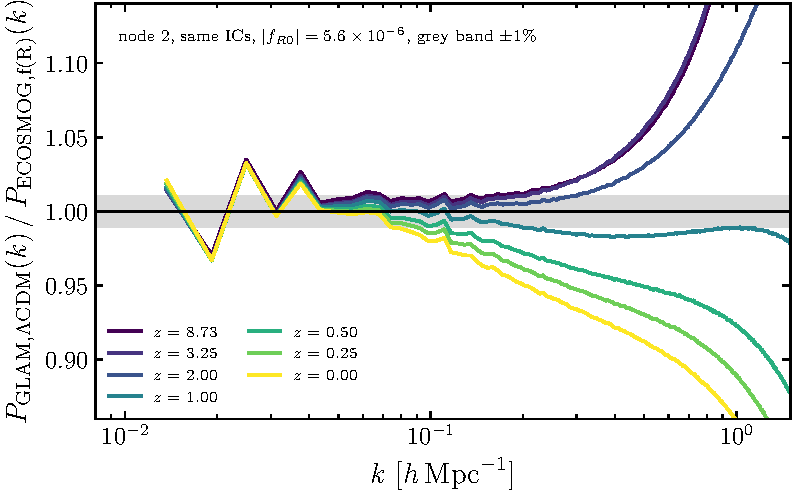
\includegraphics[width=0.60\textwidth]{figs/twin_ratio.pdf}
  \vspace{-0.5ex}
  \begin{columns}[T]
    \begin{column}{0.49\textwidth}
      \scriptsize
      \begin{itemize}
        \item Left, $\Lambda$CDM vs the f(R) twin: flat $+0.5$ to $+0.7\,\%$ at $k < 0.1$ at every epoch, already
          at $z = 8.7$; late times: ECOSMOG above us by 5\,\% ($k = 0.1$--0.3) and 10\,\% ($k = 0.3$--1), the
          f(R) enhancement for $|f_{R0}| = 5.6\times10^{-6}$.
      \end{itemize}
    \end{column}
    \begin{column}{0.49\textwidth}
      \scriptsize
      \begin{itemize}
        \item Right, f(R) vs f(R), the real twin test: the same $+0.5$ to $+0.8\,\%$ at $k < 0.1$; within $\pm1\,\%$
          to $k = 0.3$ at every epoch; $-0.6\,\%$ at $k = 0.3$--1 at $z = 0$ (PM force resolution).
          $k > 0.3$ at $z > 3$: lattice discreteness.
      \end{itemize}
    \end{column}
  \end{columns}
  \vspace{-0.5ex}
  \examplebox{The $+0.5\,\%$ at linear scales is the same in both gravity models}{%
    \scriptsize A code or ingestion offset, not physics: \texttt{ic2pm}'s half-step convention, POWMES normalisation or
    a 0.25\,\% growth difference; a $\mathrm{d}a_0 = 3\times10^{-4}$ restart of 20 steps isolates the half-step term.
  }
\end{frame}

% -----------------------------------------------------------------------------
\begin{frame}{\textbf{f(R) pilot (job 12180110): completed and verified}}
  \begin{columns}[T]
    \begin{column}{0.50\textwidth}
      \scriptsize
      \begin{tabular}{@{}lp{0.64\textwidth}@{}}
        \toprule
        & f(R), extras on \quad ($\Lambda$CDM pilot) \\
        \midrule
        wall, 64 cores & 6 h 08 min (2 h 32 min) \\
        CPU efficiency & 83\,\% (83\,\%) \\
        MaxRSS & 177 GB (118 GB) \\
        non-output step & 1.72 min; multigrid 1.1 min (0.60 min) \\
        station output & $+0.37$ min: P(k), planes ($+0.36$) \\
        primary output & $+2.9$ min: BDM + extras ($+2.0$, BDM) \\
        42 outputs & 59 min = 16\,\% of the run (29\,\%) \\
        disk per box & 25 GB (9.1 GB) \\
        \bottomrule
      \end{tabular}
    \end{column}
    \begin{column}{0.48\textwidth}
      \footnotesize
      \begin{itemize}
        \item \texttt{check\_run.py}: 42 exact outputs, 42 P(k) + planes, 17 catalogues, 0 FAIL, 0 WARN.
        \item Per primary: $\delta_m$ cube $n = 244$ (469 MB), momentum cubes $n = 162$ ($3\times138$ MB),
          subsample of $10.74$ M particles $= N/100$ to 0.03\,\%, no clipping (129 MB), $f_R$ at 1.12 M haloes
          at $z = 1$ (9 MB): 1.0 GB.
        \item V9: the extras cost at most 1.4 min per primary (the excess over the $\Lambda$CDM primaries),
          $\le 23$ min $= 6\,\%$ of this run and $\le 15\,\%$ of a $\Lambda$CDM run; an upper bound until
          \texttt{ExtraOutputs} gets per-product timers. Memory 177 GB on a 1 TB node.
        \item $\approx 390$ core-hours per f(R) box at $1024^3$.
        \item Caveats: $k_{c,\rm mom} = 1.0$ (use the momentum modes below $0.78\,h\,\mathrm{Mpc}^{-1}$);
          the binaries predate the review fixes.
      \end{itemize}
    \end{column}
  \end{columns}
\end{frame}

% -----------------------------------------------------------------------------
\begin{frame}{\textbf{Independent review: six reviewers, eight majors, all fixed}}
  \begin{columns}[T]
    \begin{column}{0.40\textwidth}
      \scriptsize
      \begin{tabular}{@{}lcccc@{}}
        \toprule
        review & B & M & m & n \\
        \midrule
        1 Fortran extras module & 0 & 0 & 9 & 5 \\
        2 scheduler, parameters, build & 0 & 2 & 6 & 6 \\
        3 particle subsample & 0 & 1 & 4 & 6 \\
        4 $\delta_L$ generator dump & 0 & 0 & 7 & 7 \\
        5 Python tools and tests & 0 & 2 & 10 & 6 \\
        6 docs and provenance & 0 & 3 & 11 & 8 \\
        \bottomrule
      \end{tabular}
      \\[1ex]
      \scriptsize Self-contained prompts and findings in \texttt{docs/reviews/degrace-track-a/}; rerunnable.
    \end{column}
    \begin{column}{0.58\textwidth}
      \footnotesize
      \textbf{Majors and their fixes}
      \begin{itemize}
        \item subsample ``ID'' was the IC file order $\to$ \texttt{ic2pm} scatters by Gadget ID and tags the lattice order
        \item optional \texttt{Init.dat} lines defaulted silently when malformed $\to$ stop with the line
        \item $f_R$ gate on \texttt{MG\_flag} only $\to$ also \texttt{MG\_model = 1}
        \item twin script skipped early epochs (5-decimal header) $\to$ epochs from the schedule file
        \item no test sensitive to axis order/sign of the dumps $\to$ mode-by-mode test
        \item plan flags table, catalogue velocity epoch, interlacing status $\to$ documented, rules added
      \end{itemize}
      \textbf{After the fixes}: suite 180/180, four scripts green, merged.
    \end{column}
  \end{columns}
\end{frame}

% -----------------------------------------------------------------------------
\begin{frame}{\textbf{Decisions pending and open items}}
  \footnotesize
  \textbf{Decisions (yours)}
  \begin{itemize}
    \item \textbf{BDM catalogue velocities} are converted with $1/a$, the new products with $1/a_v$: the catalogue
      is low by $a_v/a$, $0.8\,\%$ ($z = 2$) to $0.3\,\%$ ($z = 0$). Fix the legacy finder (changes every GLAM
      catalogue) or keep documenting it (multiply by $a/a_v$ offline; \texttt{glamio} does).
    \item \textbf{Momentum deposit} at $N_g = 4096$ f(R): the transient $N_{\rm dep}^3$ buffer (34 GB) does not fit the
      985 GB runs; reuse \texttt{FI} or restrict extras to $N_g = 2048$.
    \item \textbf{Interlacing}: not implemented; default $k_{c,\rm mom} = 0.75$ stays below $k_{N,\rm dep}/4$ and
      PMP2init refuses more. Implement if $k > 0.78$ momentum modes are wanted.
    \item \textbf{Disk}: 1.5 TB freed on 17 Oct (validation IC, February checkpoints, BDM PM snapshots); still to
      decide: the 21 BDM replay density tapes and membership tapes (195 GB on disk), 15 GB of superseded fiducial catalogues.
  \end{itemize}
  \textbf{Open minors} (grouped in \texttt{TRIAGE.md}): parameter-path robustness, $f_R$ product details, provenance
  JSON, test strength, docs drift. \quad \textbf{Questions for Baojiu}: BDM cadence, plane normalisation, CAMB
  $\omega_c$ pitfall, r2g velocity convention, node 900.
\end{frame}

% -----------------------------------------------------------------------------
\begin{frame}{\textbf{Next steps}}
  \small
  \begin{enumerate}
    \item Explain the $+0.5\,\%$: the $\mathrm{d}a_0 = 3\times10^{-4}$ restart test (half-step term) and a POWMES
      normalisation check; add per-product timers to \texttt{ExtraOutputs} (the V9 split).
    \item Settle the three decisions above; rebuild the frozen pilot binaries from \texttt{cz}.
    \item Production recipe per node: \texttt{gen\_inputs.py --node N --gravity \{lcdm,fr\}} $\to$ \texttt{submit.sh}
      (\texttt{ic2pm half} on Baojiu's ICs) $\to$ \texttt{check\_run.py}; $\approx 165$ core-hours per $\Lambda$CDM box,
      $\approx 390$ for f(R); 9 GB ($\Lambda$CDM) or 25 GB (f(R) with the extras) per box.
    \item Readers for the new products in \texttt{halocat} (planes, modes, subsample, $f_R$), following the
      \texttt{.meta} keys.
    \item Reply to Baojiu with the cross-check of the 42 epochs and the open questions.
  \end{enumerate}
\end{frame}

% -----------------------------------------------------------------------------
\begin{frame}{\textbf{Summary}}
  \small
  \begin{itemize}
    \item The DEGRACE companion outputs (schedule, lens planes, $\delta_L$, modes, subsample, $f_R$) are implemented,
      tested, reviewed and merged into \texttt{cz}.
    \item The $\Lambda$CDM pilot runs in 2.5 h per box with all 42 outputs, the f(R) pilot with all the extras
      in 6 h; the new products cost about 1\,\% of a run, the halo finder 23\,\%, the extras at most 6\,\%.
    \item Both pilots agree with the ECOSMOG twin to $+0.5$--$0.8\,\%$ at linear scales at every epoch, and the
      f(R) run reproduces the f(R) spectrum to $\pm1\,\%$ up to $k = 0.3$; the small constant offset is common
      to both gravity models and is the one question still open.
    \item Three design decisions stand between here and production.
  \end{itemize}
\end{frame}

\end{document}
